\documentclass[conference]{IEEEtran}
\IEEEoverridecommandlockouts
% The preceding line is only needed to identify funding in the first footnote. If that is unneeded, please comment it out.
\usepackage{cite}
\usepackage{amsmath,amssymb,amsfonts}
\usepackage{algorithmic}
\usepackage{graphicx}
\usepackage{textcomp}
\usepackage{xcolor}
\def\BibTeX{{\rm B\kern-.05em{\sc i\kern-.025em b}\kern-.08em
    T\kern-.1667em\lower.7ex\hbox{E}\kern-.125emX}}
\begin{document}

\title{Sistema de información visual \\para pasajeros de trenes argentinos}


\author{\IEEEauthorblockN{Carlos German Carreño Romano}
\IEEEauthorblockA{\textit{Universidad de Buenos Aires}\\
\textit{(UBA) Facultad de Ingeniería}\\
Buenos Aires, Argentina\\
ccarreno@fi.uba.ar}
\and
\IEEEauthorblockN{Pablo Martín Gomez}
\IEEEauthorblockA{\textit{Universidad de Buenos Aires}\\
\textit{(UBA) Facultad de Ingeniería}\\
\textit{(LSE) Laboratorio de Sistemas Embebidos}\\
Buenos Aires, Argentina\\
pgomez@fi.uba.ar}
}



\maketitle

\begin{abstract}
En los trenes existen distintos sistemas de control que se interconectan por medio de una red de comunicaciones del tren (TCN). Algunos ejemplos son el sistema de frenos, el control de puertas, el aire acondicionado y el sistema de información visual al pasajero (PIDS). El PIDS es el responsable de transmitir mensajes como el destino o la próxima estación usando carteles de matriz led y tiene su propia red. También incluye mapas con indicadores led, un sistema de audio y un circuito cerrado de cámaras. El propósito de este trabajo es desarrollar firmware y hardware necesarios para controlar los carteles de matriz LED de salón (IDU) de las formaciones ferroviarias de Trenes Argentinos. El principal valor que aporta es generar herramientas de mantenimiento para extender la vida útil de los trenes. Si bien existen carteles led comerciales de propósito general, en los trenes hace falta conectarlos a la red, interpretar datos y protocolos del PIDS, presentar mensajes en función de los datos y considerar restricciones eléctricas. En el diseño e implementación del sistema embebido de este trabajo se aplicaron patrones de software concurrente (máquinas de estado y objeto activo) usando un sistema operativo de tiempo real (RTOS) sobre una plataforma EDU-CIAA. También se desarrollaron piezas de hardware para adaptar el sistema a la red y se realizaron capturas de tramas de datos en formaciones ferroviarias operando en vivo.\\

\end{abstract}


\begin{IEEEkeywords}
TCN, PIDS, RTOS, EDU-CIAA, Trenes Argentinos
\end{IEEEkeywords}

\section{Introducción}

El uso de carteles de matriz led, además de ser usados en trenes, está extendido a aplicaciones como los sistemas de información en aeropuertos, en paradas de ómnibus, en señalamiento vial y en la industria del entretenimiento. Las dimensiones del cartel, la densidad de píxeles por unidad de área, la cantidad de colores o leds por píxel, los niveles de intensidad lumínica, el brillo y contraste, la potencia eléctrica, son algunas de las especificaciones típicas. Los controladores pueden basarse en circuitos digitales, en microcontroladores de 8, 16 o 32 bits, en FPGA, y existe diversidad en la implementación del software embebido. El envío de datos y el formato de los mismos dependen de la implementación. \\

En \cite{b1} se utiliza el chip AT89C52 para enviar caracteres chinos sobre matrices de 32 x 192 leds de un solo color; en \cite{b2} se implementa una pantalla led RGB de 320 x 240 píxeles que rota 360º permitiendo visualizar imágenes en color por persistencia de visión; en \cite{b3} se desarrollan algoritmos sobre FPGA usando búferes de datos para controlar una pantalla LED de 160 x 32 píxeles alcanzando 32,768 colores; en \cite{b4} se presenta el control de un micro display de transistores de película delgada (TFT) usando modulación por ancho de pulso (PWM) alcanzando 256 niveles de color a una frecuencia de refresco de 60 Hz, basado también en FPGA; en \cite{b5} se presenta el control de píxeles virtuales para matrices led multicolor usando flip-flops tipo D. \\

En el diseño e implementación del presente trabajo, los carteles son de matriz led de un solo color y de distintas dimensiones (8x64, 32 x 64, 32 x 128). El control de los carteles tiene como factor común el uso del conjunto de chips digitales 74HC138, 74HC595 y 74HC245. La topología permite interconectar paneles en serie para construir carteles led de distinto tamaño usando la misma lógica de control. \\

\subsection{Introducción específica}

El sistema PIDS de las formaciones de Trenes Argentinos (SOFSE) adquiridas en 2015 tiene una arquitectura propietaria que usa una red física RS485 más una serie de protocolos definidos por el fabricante para cada interfaz. Cabe mencionar que desde 2008 \cite{b6} la IEC busca desarrollar estándares para TCN usando redes Ethernet de tiempo real. En 2016 se publica  IEC62580-2 que incluye al sistema de información al pasajero (ahora llamado PIS), el CCTV y los protocolos asociados en el estándar. Sin embargo, este nuevo estándar no estaría disponible en dispositivos comerciales hasta finales de 2016-2017. El estudio y desarrollo de herramientas de mantenimiento para la red PIDS existente es de gran relevancia para el personal de trenes argentinos, porque permite extender la vida útil de los trenes planificada en no menos de 20 años y además reducir la dependencia tecnológica con los fabricantes. En este trabajo se estudia entonces el sistema PIDS basado en redes RS485 con protocolos.\\

El propósito de este trabajo es desarrollar el firmware y hardware necesarios para controlar los carteles LED de salón de formaciones ferroviarias de Trenes Argentinos. Los carteles forman parte del sistema PIDS, una red RS485 que se interconecta a la red de comunicaciones del tren TCN. La red TCN presenta una arquitectura de buses jerárquicos de dos niveles, el bus de datos WTB y el MVB \cite{b7}. En la figura \ref{fig.embeddedSystem} se representan los buses de la red TCN, y el sistema embebido propuesto para conectar los carteles LED al sistema.\\


\begin{figure}[htbp]
\centerline{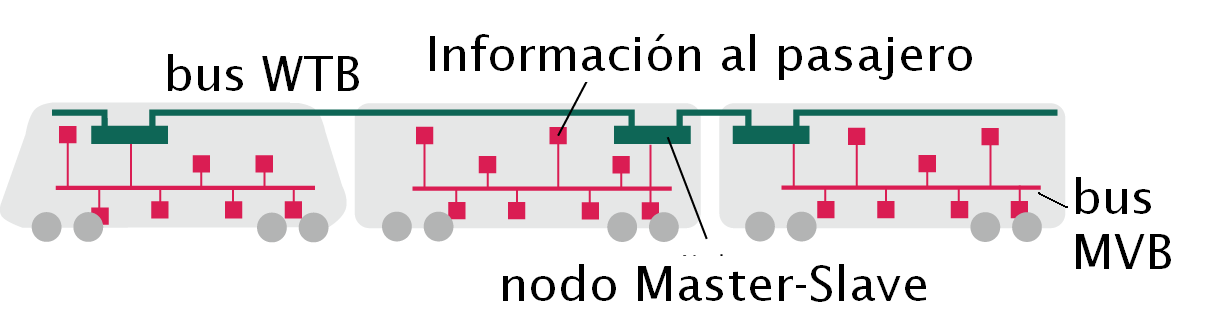
\includegraphics[width=0.4\textwidth]{diagramaRedTCN.png}}
\vspace{0.4cm}
\centerline{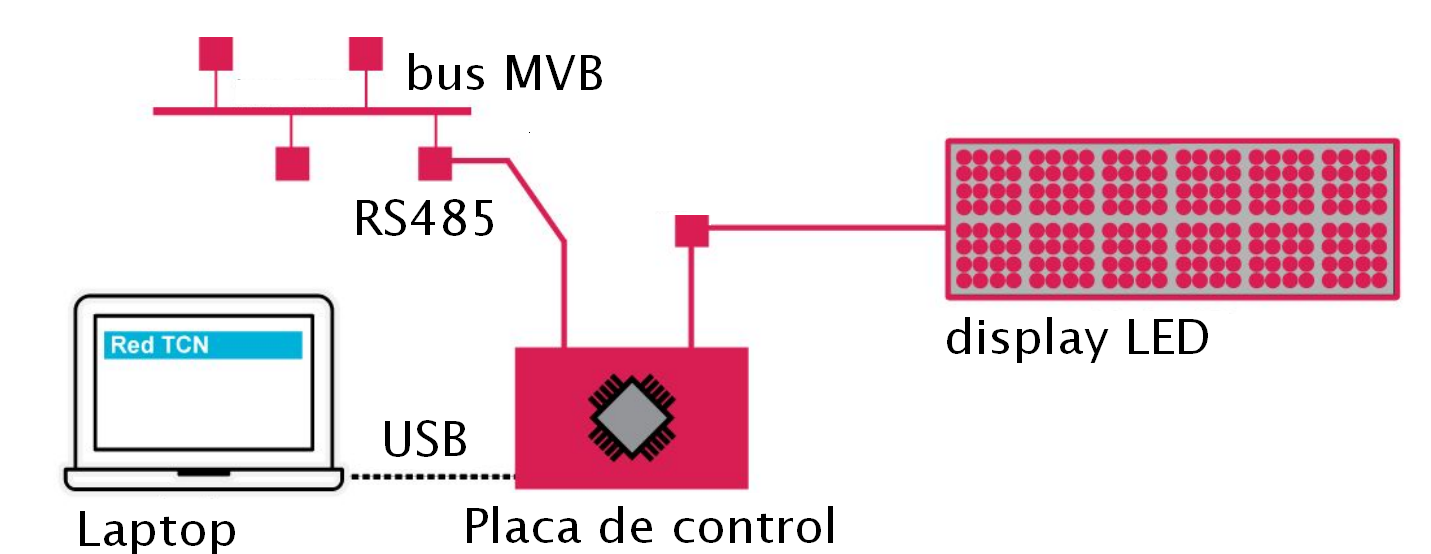
\includegraphics[width=0.5\textwidth]{diagramaPIDSCIAA.png}}
%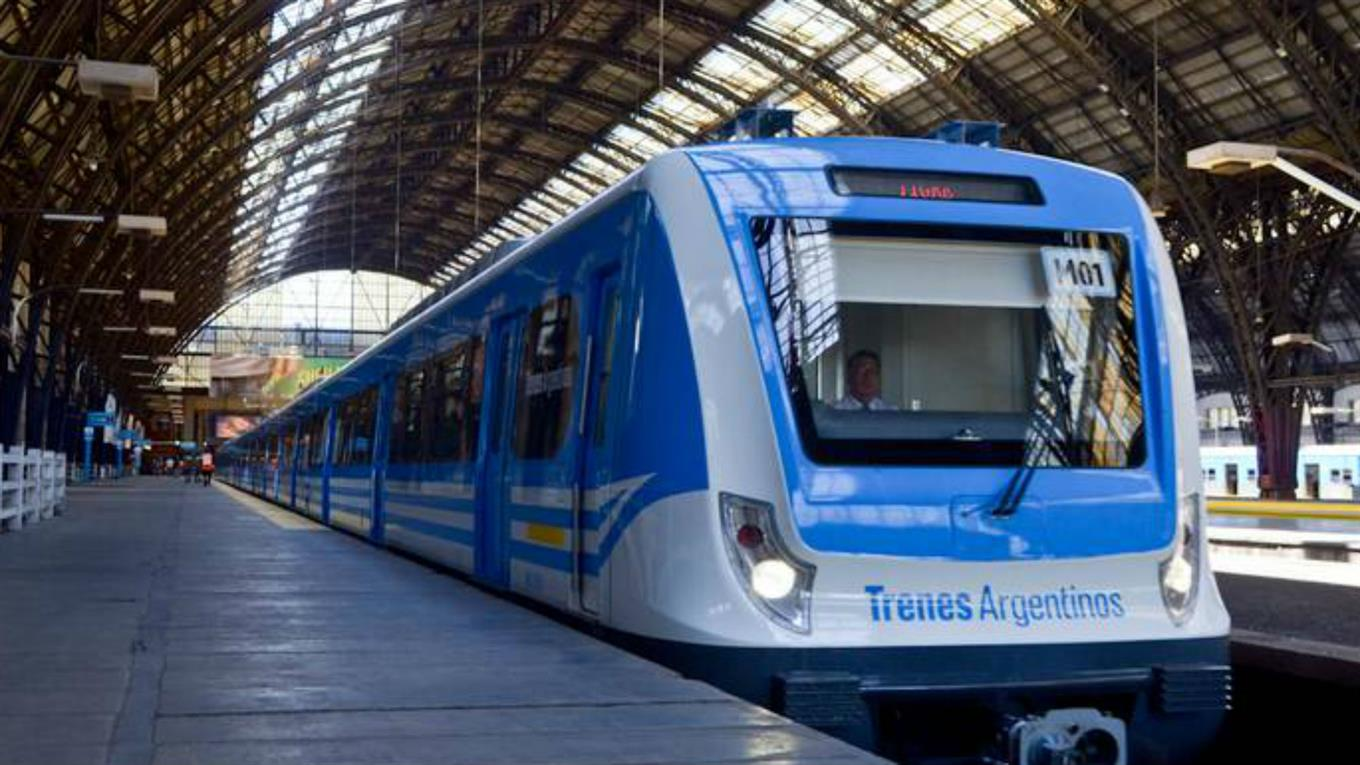
\includegraphics[width=.75\textwidth]{./Pics/tren.jpg}
\caption{Arriba: diagrama de los buses de datos WTB y MVB de la red TCN. Abajo: diagrama del sistema embebido propuesto para controlar los carteles LED de salón. El sistema se compone de la placa de control y su firmware, las interfaces con el cartel led, con la red RS485 y con una laptop.}
\label{fig.embeddedSystem}
\end{figure}


\section{Desarrollo}

Para estudiar la comunicación entre estos buses de datos se desarrollaron piezas de hardware y software que permiten capturar paquetes de la red RS485. En la figura  \ref{fig.fotosTren} se puede observar la conexión realizada en las formaciones de SOFSE para la captura de datos de la red PIDS en operación.\\

\begin{figure}[htbp]
\centerline{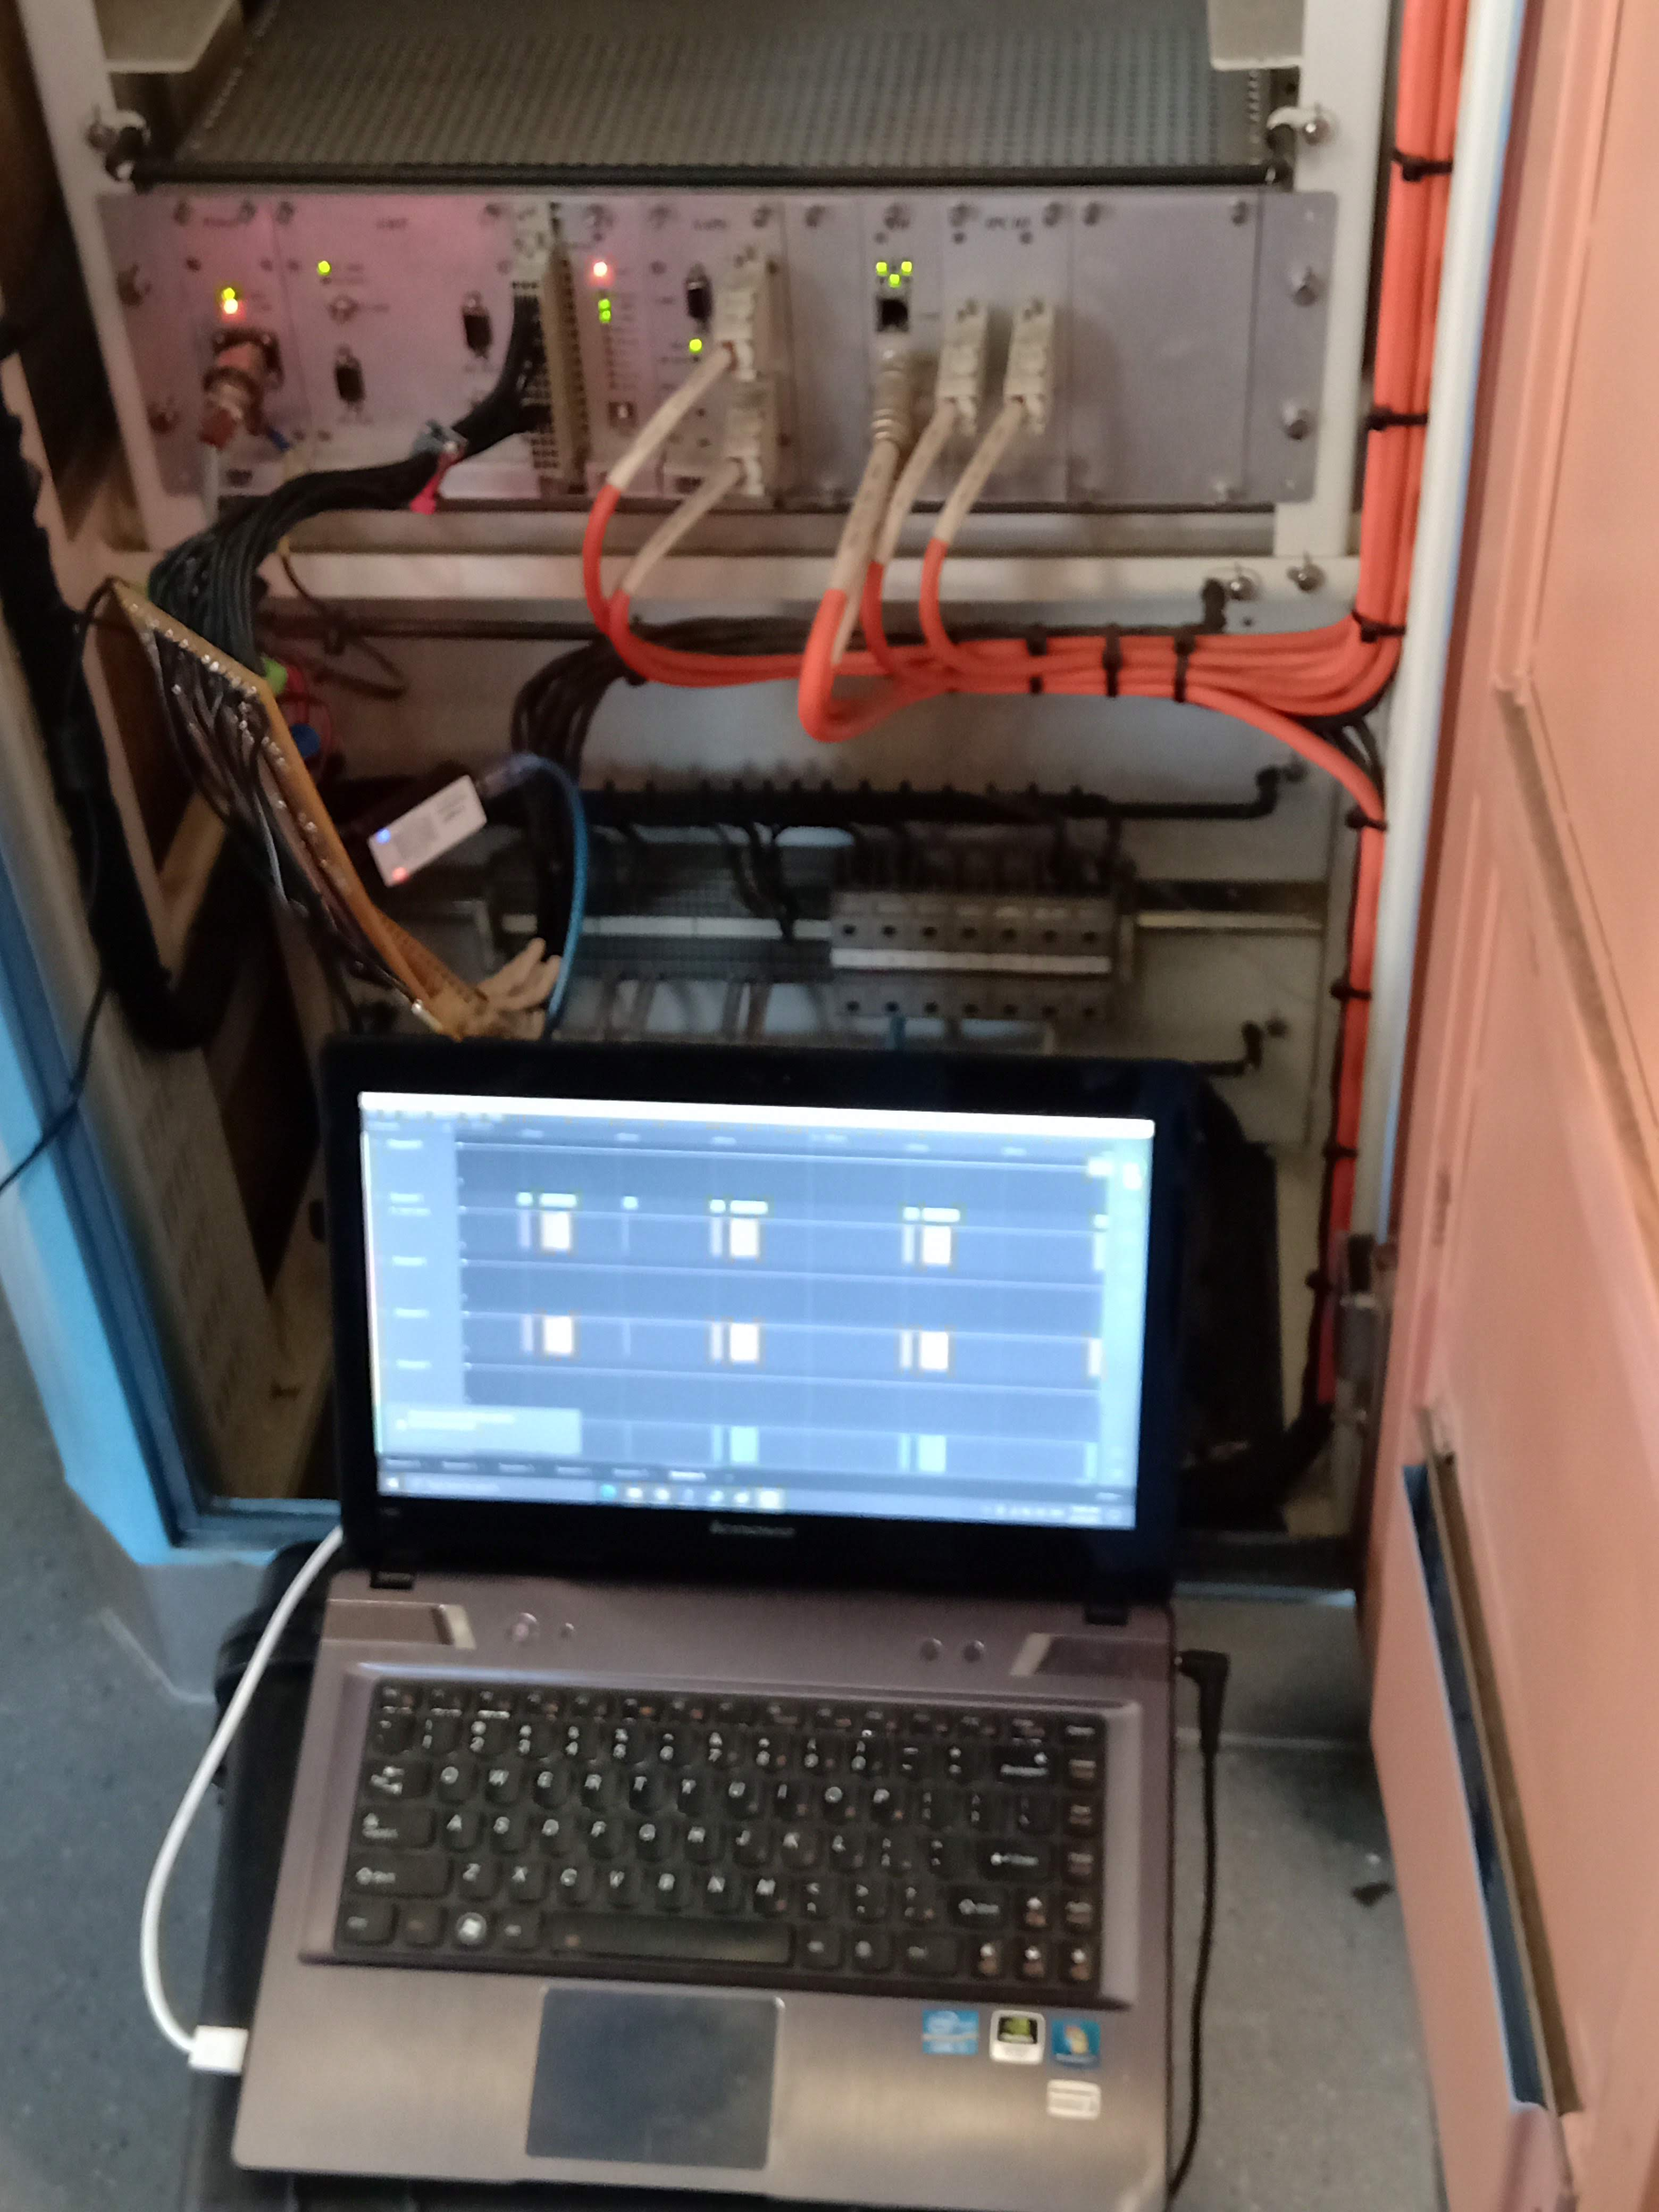
\includegraphics[width=0.45\textwidth]{fotoSetupTren.jpg}}
\vspace{0.4cm}
\centerline{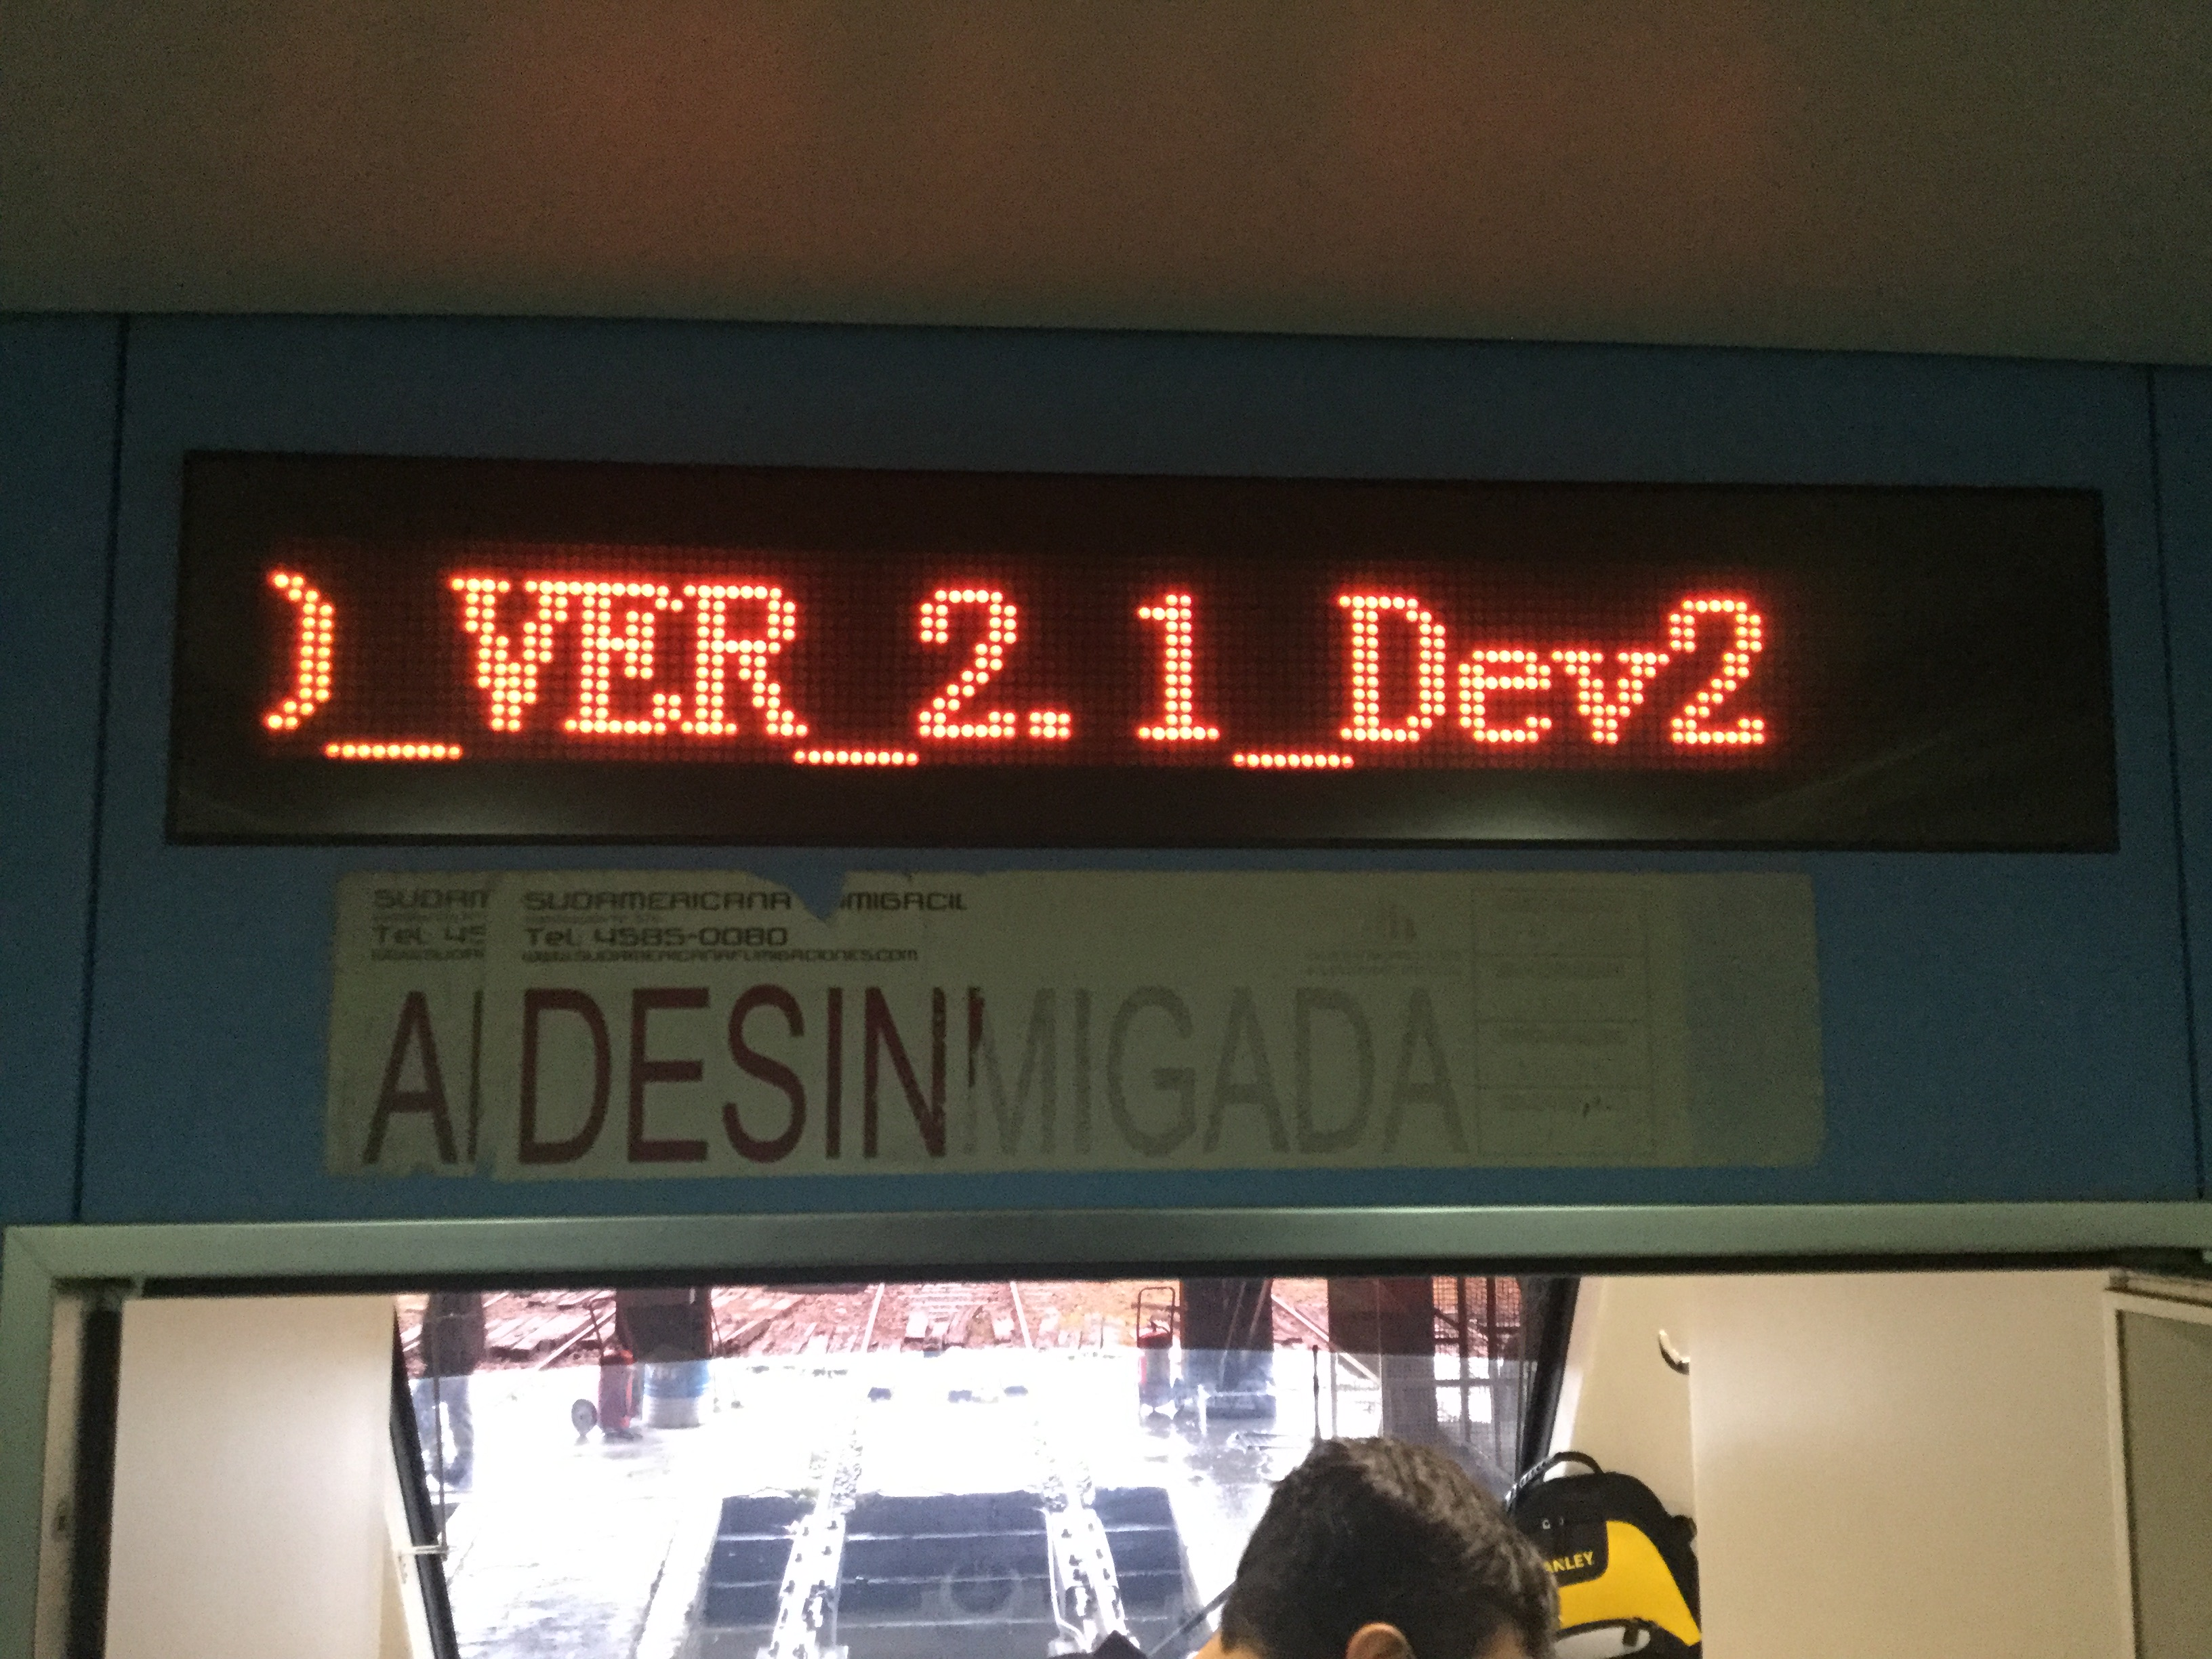
\includegraphics[width=.45\textwidth]{fotoCartelSalon.JPG}}
\caption{Arriba: Fotografía de las mediciones realizadas sobre la red PIDS. Abajo: Cartel LED de salón inicializándose.}
\label{fig.fotosTren}
\end{figure}

Estas tramas de datos se estudiaron posteriormente logrando identificar patrones. Las mediciones buscan identificar la comunicación entre los carteles de matriz led y el resto del sistema. \\

\subsection{Diseño e implementación de sistema embebido}

El sistema embebido del presente trabajo debe resolver la comunicación entre la red RS485 del sistema PIDS y los carteles LED de salón. La placa de control está basada en la plataforma EDU-CIAA. La misma se puede comunicar con una computadora personal y tiene la función de recibir datos de la red RS485 y presentar  información al pasajero a través de los carteles LED.\\

\subsection{Casos de uso}
Los casos de uso requeridos del sistema involucran al tren, al operador o conductor de tren, al sistema y a los pasajeros. Cuando el tren arriba a una estación se debe presentar información visual al pasajero. Si el conductor presiona un botón, el sistema debe también presentar información predeterminada al pasajero, por ejemplo las estaciones cabecera del recorrido que se visualizan en los carteles LED de frente y contrafrente del tren. Cierta información, por ejemplo de prevención, se puede presentar al pasajero periódicamente. Este caso de uso implica eventos temporales mientras el tren está en circulación.\\

 Por último, un caso de uso de particular interés es decodificar las tramas de datos que viajan por la red PIDS para alimentar un sistema externo, por ejemplo un sistema de transmisión de datos del tren a la nube, o una herramienta local de chequeo de datos.  Este es un caso de uso en el que el cliente no es un pasajero sino otro sistema. \\

\subsection{Patrones}
Los casos de uso plantean problemas de diseño a resolver que presentan similitudes. En los casos de presentar información visual al pasajero el problema a resolver implica observar variables de estado y generar mensajes de salida en base a algún criterio. Se utiliza para estos casos el patrón observar y reaccionar \cite{b8}. En sistemas embebidos también es usual utilizar el patrón máquina de estados finitos (fsm) \cite{b9}. Este es un patrón de comportamiento que permite actualizar el estado interno de un objeto como respuesta a entradas. En cada momento la fsm puede estar en un sólo estado posible, y las transiciones entre estados están normalmente asociadas a eventos. En este trabajo se realiza una implementación de fsm utilizando un arreglo de estructuras y handlers usando punteros a función \cite{b10}. \\

Dado que el sistema tiene como requerimientos dar respuesta a eventos de forma asincrónica, se hará uso también del patrón objeto activo (AO)\cite{b11}. Este es un patrón que permite desacoplar los métodos de invocación y ejecución para mejorar la concurrencia y simplificar el acceso a datos de un objeto que tiene su propio hilo de control. El patrón AO se utiliza en este trabajo usando una implementación en C sobre RTOS que permite a cada tarea ejecutar una máquina de estados en un ciclo infinito  \cite{b12}, estandarizando la interfaz entre tareas por medio de una cola FIFO. Las tareas esperan por nuevos eventos a ser procesados usando esta interfaz, y mientras no reciban eventos se mantienen en estado inactivo. Cuando se recibe un evento, RTOS despierta la tarea y ésta ejecuta una actualización en la máquina de estados asociada. \\

En este sistema se hará uso del patrón AO para simplificar el acceso a distintas máquinas de estado que deberán funcionar de forma concurrente. La solución que se plantea en este documento hace uso de estos patrones de forma combinada.\\


\subsection{Firmware}



Los datos de entrada de la red RS485 se reciben usando la interfaz UART. Se ha programado esta interfaz usando interrupciones (ISR UART) como se indica en la figura \ref{fig.fsm}(a). La interrupción está configurada para usar un callback (IRQ UART) que otorga un semáforo de RTOS. Este semáforo es tomado siempre por una tarea de RTOS (vTask UART) que se encarga de leer los datos de entrada y encolar mensajes de eventos para actualizar una máquina de estados. Este mecanismo logra que la rutina de interrupción sea muy corta, permitiendo una buena performance en términos de tasa de datos, modularidad y simplicidad. La tarea de leer los bytes de entrada y de resolver una acción concreta quedan desacopladas usando objeto activo.\\

 En la figura \ref{fig.fsm} se presentan los diagramas de dos de los objetos activos implementados en el firmware del sistema embebido desarrollado.\\

\begin{figure}[htbp]
\centerline{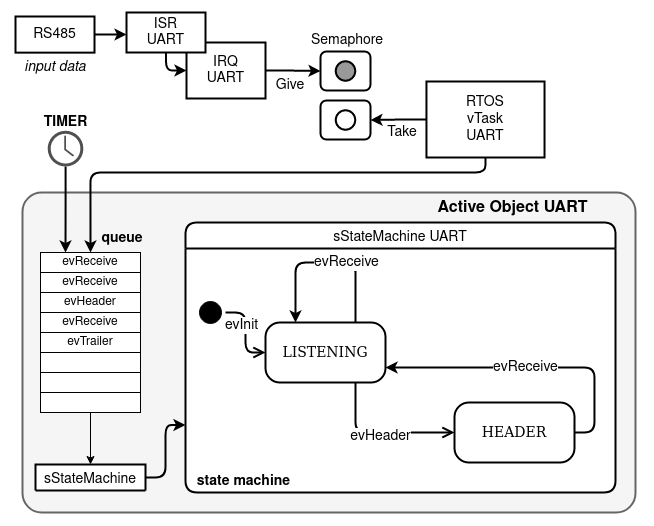
\includegraphics[width=0.45\textwidth]{fsmUART2.png}}
\vspace{0.4cm}
\centerline{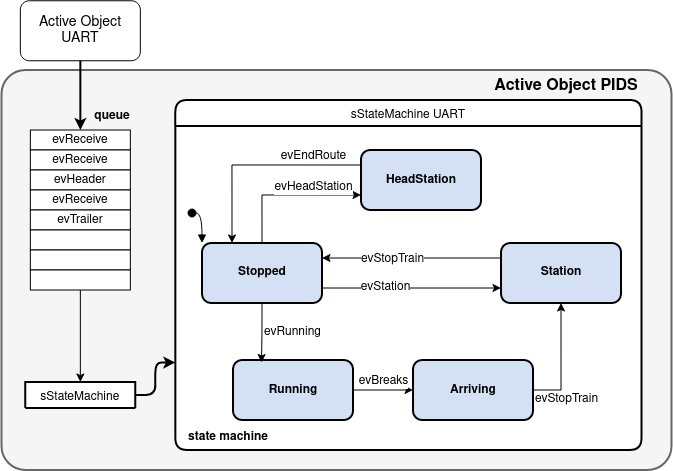
\includegraphics[width=0.45\textwidth]{fsmTrain.png}}
%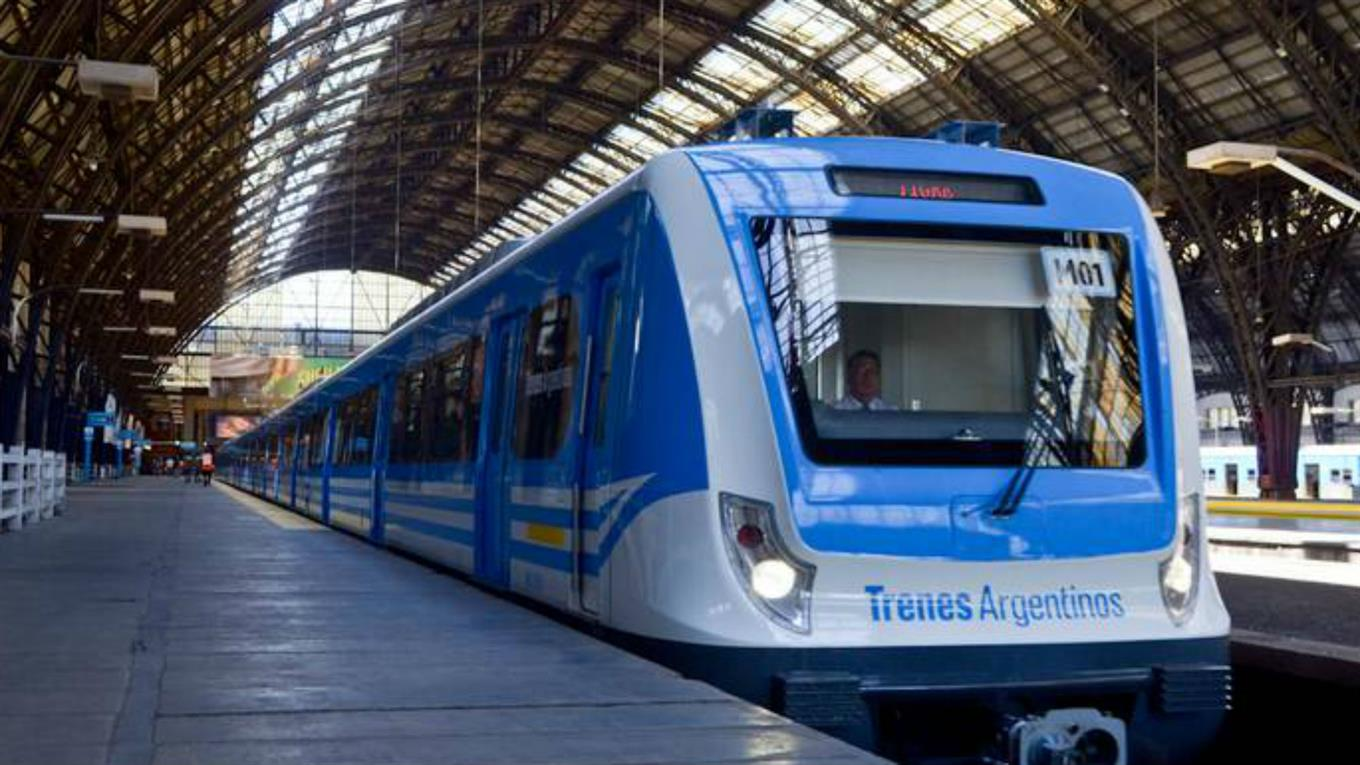
\includegraphics[width=.75\textwidth]{./Pics/tren.jpg}
\caption{(a) Arriba: diagrama del objeto activo que maneja la UART y usando RTOS. (b) Abajo: el diagrama del objeto activo que administra el contexto, es decir el estado del tren.}
\label{fig.fsm}
\end{figure}

El manejo de la lógica asociada al tren también se resuelve con un objeto activo que administra otra máquina de estados. En particular, esta última se puede ver en la figura \ref{fig.fsm}(b) y representa los estados de circulación del tren, siendo la que guarda relación directa con el contexto. Cuando el tren está en circulación, una serie de sensores envían datos de entrada que serán procesados y se recibirá un mensaje por la cola FIFO. Si el tren frena, la máquina de estados debe pasar al estado detenido (Stopped). En cada uno de estos estados se guarda un mensaje de información visual predeterminado. Estos mensajes se pueden configurar modificando un archivo en el firmware. \\


\subsection{Pruebas de validación}

Para realizar pruebas del sistema se ha montado una maqueta que se pueda observar en la figura \ref{fig. foto Cartel home}. Esta maqueta está formada por la EDU-CIAA, un adaptador de conectores de 2x8 pines y la placa del display led. La EDU-CIAA está conectada a una computadora personal, recibiendo datos por la interfaz UART y enviando datos al cartel usando pines de salido GPIO. \\

\begin{figure}[htbp]
\centerline{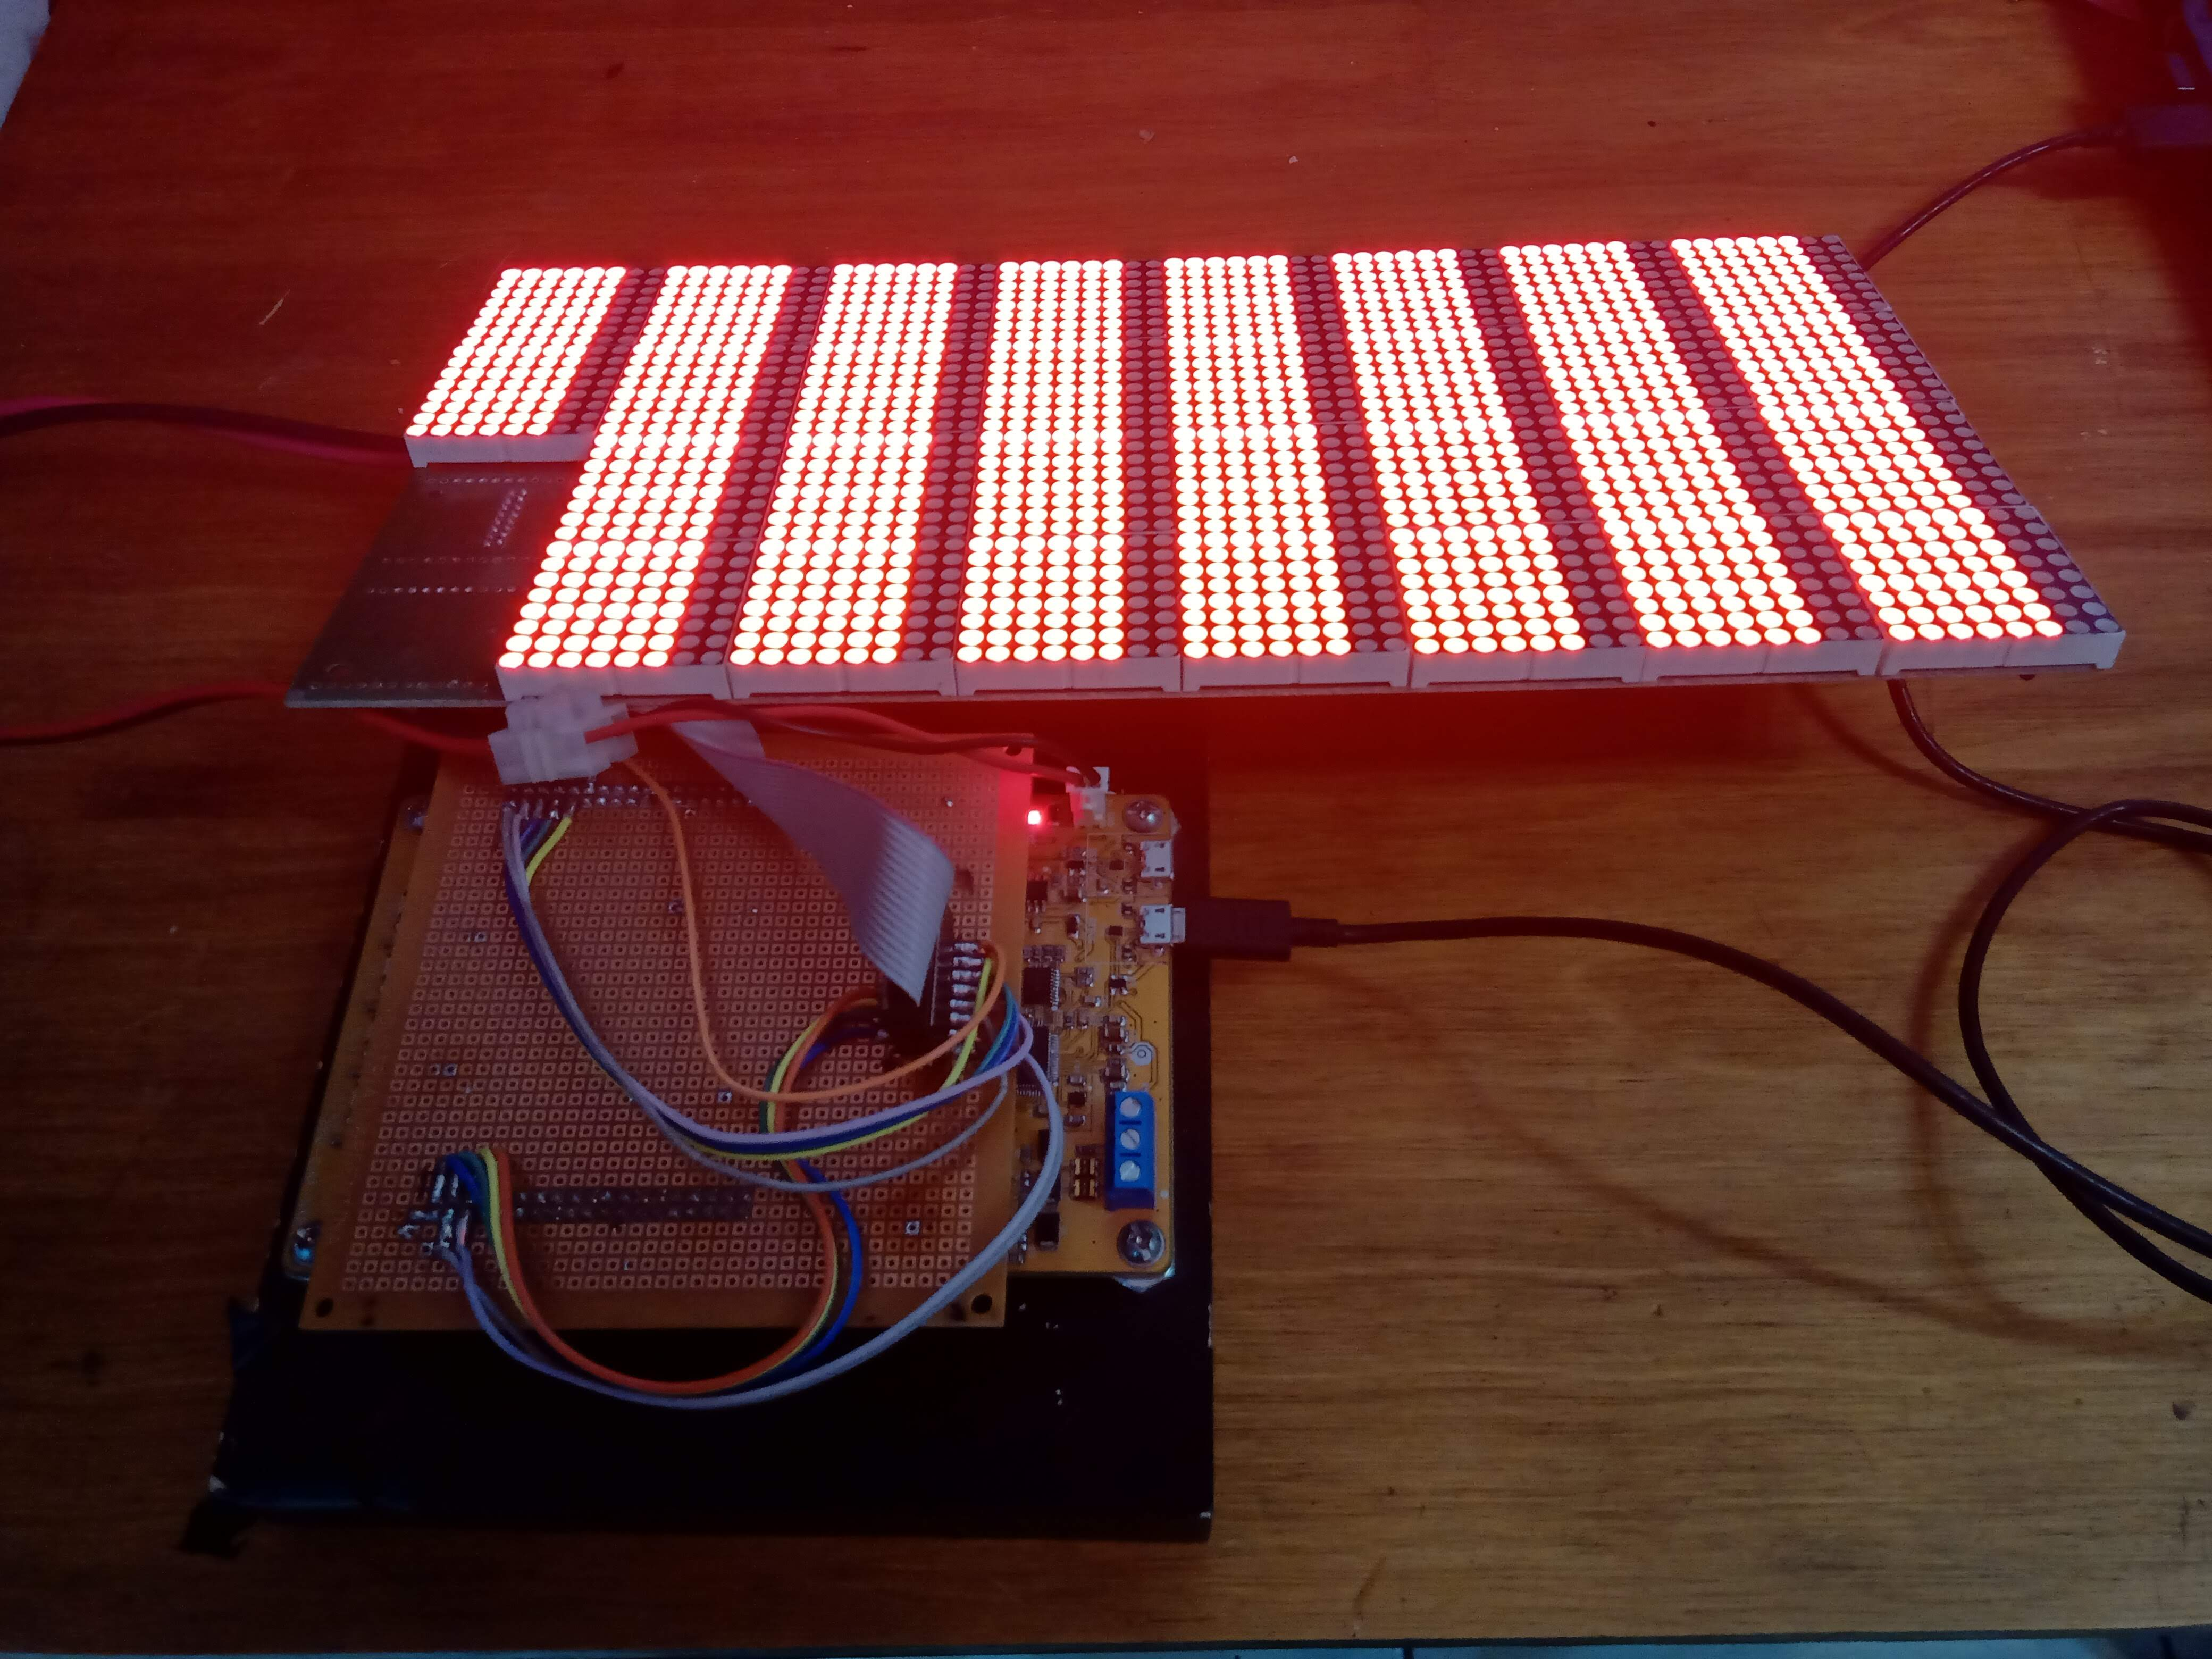
\includegraphics[width=0.45\textwidth]{fotoCartelTest.jpg}}
%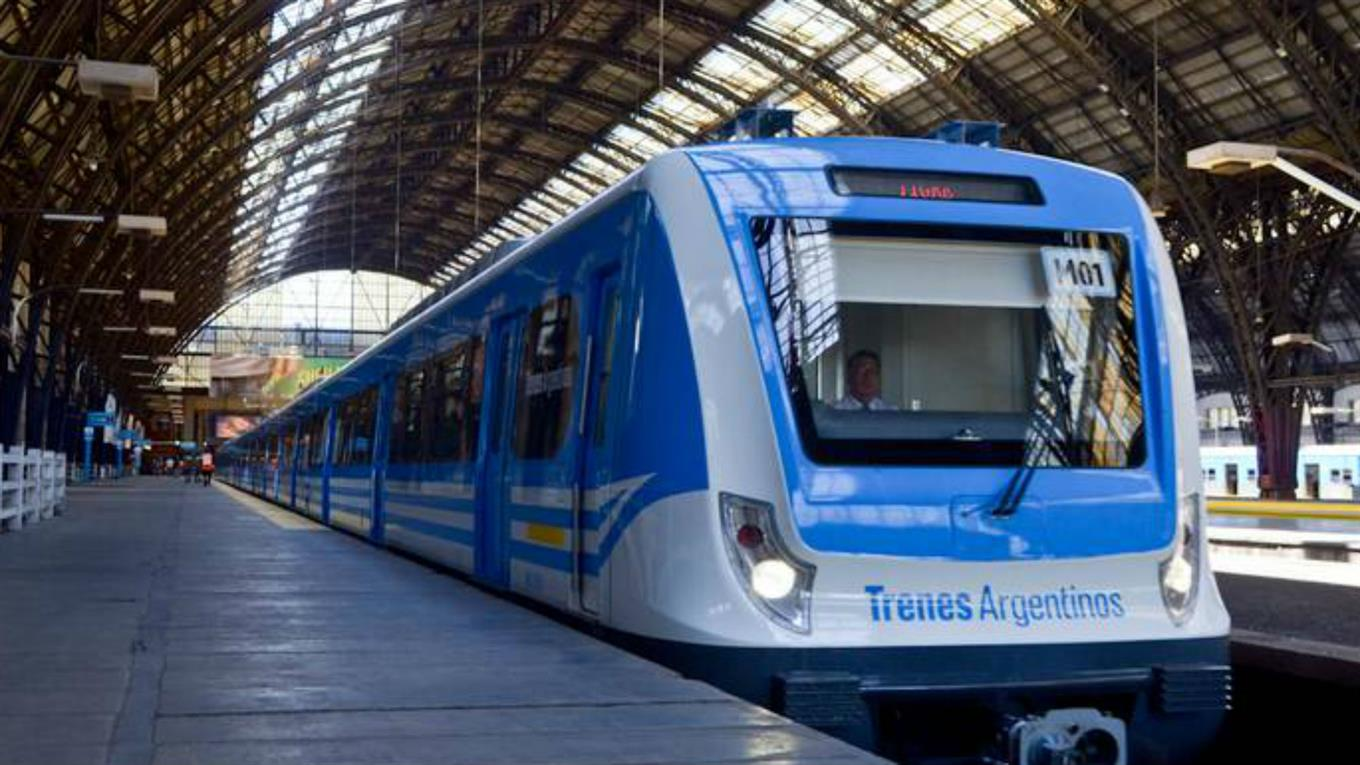
\includegraphics[width=.75\textwidth]{./Pics/tren.jpg}
\caption{Fotografía de la maqueta para testear el control del cartel de matriz led usando la plataforma EDU-CIAA y un adaptador.}
\label{fig. foto Cartel home}
\end{figure}

Las pruebas realizadas permiten validar el firmware desarrollado para controlar carteles de matriz led compatibles con los existentes en las formaciones de SOFSE.\\


\section{Conclusiones}

Este trabajo en progreso en colaboración con Trenes Argentinos permite estudiar los protocolos de la red PIDS y la comunicación con los carteles led de salón. Se han desarrollado piezas de hardware y software que funcionan como herramientas de mantenimiento. El control de los carteles de matriz led usando el conjunto de chips descrito es escalable, de bajo costo, y de complejidad media en el manejo de señales digitales. Estos carteles pueden ser candidatos a fabricación en serie. Se ha logrado controlar estos carteles usando la plataforma EDU-CIAA. Se ha observado que por las tramas de datos de la red PIDS no viajan mensajes, sino códigos asociados a dispositivos. Cada dispositivo, como un cartel led, está nomenclado con una dirección. Las placas de control que funcionan como interfaz entre la red RS485 y los carteles led de salón se alimentan de entradas de corriente continua de 110 V. Distintos módulos adaptadores de tensión permiten el funcionamiento de un circuito de datos basado en un microcontrolador de 32 bits. Esta observación es la que permite y da sentido a este desarrollo ya que el prototipo desarrollado permitiría reemplazar las placas del fabricante por hardware de fabricación nacional, reduciendo de esta manera la dependencia tecnológica y acortando las cadenas de suministro.



\begin{thebibliography}{00}
\bibitem{b1} SONG, Yongxian, et al. Design of LED Display Control System Based on AT89C52 Single Chip Microcomputer. J. Comput., 2011, vol. 6, no 4, p. 718-724.

\bibitem{b2} LIU, Shih-Mim; CHEN, Ching-Feng; CHOU, Kuang-Chung. The design and implementation of a low-cost 360-degree color LED display system. IEEE transactions on consumer electronics, 2011, vol. 57, no 2, p. 289-296.

\bibitem{b3} KURDTHONGMEE, W. Design and implementation of an FPGA-based multiple-colour LED display board. Microprocessors and Microsystems, 2005, vol. 29, no 7, p. 327-336.

\bibitem{b4} LIN, Yi-Zhen, et al. Active-matrix micro-LED display driven by metal oxide TFTs using digital PWM method. IEEE Transactions on Electron Devices, 2021, vol. 68, no 11, p. 5656-5661.

\bibitem{b5} GAGO, Alfonso; FERNÁNDEZ, José; BOHÓRQUEZ, Alfonso G. Control architecture of a virtual matrix LED display without current drivers. En 2009 International Symposium on Intelligent Signal Processing and Communication Systems (ISPACS). IEEE, 2009. p. 53-56.


\bibitem{b6} Feng, Jianghua, et al. "Survey of development and application of train communication network." Proceedings of the 2015 International Conference on Electrical and Information Technologies for Rail Transportation. Springer, Berlin, Heidelberg, 2016.

\bibitem{b7} Schifers, C., and Gernot Hans. "IEC 61375-1 and UIC 556-international standards for train communication." VTC2000-Spring. 2000 IEEE 51st Vehicular Technology Conference Proceedings (Cat. No. 00CH37026). Vol. 2. IEEE, 2000.

\bibitem{b8} Sommerville, Ian. "Software Engineering 10." Harlow: Pearson Education Limited (2016).

\bibitem{b9} Lavender, R. Greg, and Douglas C. Schmidt. "Active object--an object behavioral pattern for concurrent programming." (1995).

\bibitem{b10} Samek, Miro. Practical UML statecharts in C/C++: event-driven programming for embedded systems. CRC Press, 2008.

\bibitem{b11} https://aticleworld.com/state-machine-using-c/, consultado en Junio 2022.

\bibitem{b12} https://www.sinelabore.de/doku.php/wiki/howto/rtos, consultado en Junio 2022.

\bibitem{b8} Introduction to Driving LED Matrices, Application Note 1216, Avago Technologies.


\end{thebibliography}

\end{document}
